\documentclass[border=4pt]{standalone}
\usepackage{amsmath,amssymb,amsfonts}
\usepackage{xcolor,colortbl,array,booktabs,multirow}
\usepackage{tikz}
\usepackage{pgfplots}
\pgfplotsset{compat=1.16}
\usetikzlibrary{arrows, automata, backgrounds, calendar, chains, decorations,
    matrix, mindmap, patterns, petri, positioning, shadows, shapes.geometric,
    trees, shapes, decorations.pathreplacing, calc, tikzmark, arrows.meta,
    intersections, fit, graphs, quotes, angles, decorations.markings}
\newcommand{\st}{\text{ s.t. }}
\newcommand{\x}{\mathbf{x}}
\renewcommand{\b}{\mathbf{b}}
\renewcommand{\c}{\mathbf{c}}
\newcommand{\A}{\mathbf{A}}
\newcommand{\y}{\mathbf{y}}
\newcommand{\z}{\mathbf{z}}
\newcommand{\R}{\mathbb{R}}
\newcommand{\RR}{\mathbb{R}}
\newcommand{\Z}{\mathbb{Z}}
\newcommand{\ZZ}{\mathbb{Z}}
\newcommand{\npcomplete}{NP-complete}
\providecommand{\true}{\text{TRUE}}
\providecommand{\false}{\text{FALSE}}
\tikzset{vertex/.style={circle,fill=black!25,minimum size=20pt,inner sep=0pt},
    edge/.style={draw,thick,-},weight/.style={font=\small},
    selected vertex/.style={vertex, fill=red!24},
    selected edge/.style={draw,line width=2pt,-,red!50},
    ignored edge/.style={draw,line width=2pt,-,black!20}}
\newcommand{\vect}{\vec}
\providecommand{\ds}{\displaystyle}
\providecommand{\longvect}{\overrightarrow}
\usepackage[normalem]{ulem}
\definecolor{ocre}{RGB}{243,102,25}
\providecommand{\leftB}{\left[}
\providecommand{\rightB}{\right]}
\tikzset{directed/.style={postaction={decorate,decoration={markings,mark=at position .65 with {\arrow{>}}}}},
    directed1/.style={postaction={decorate,decoration={markings,mark=at position .65 with {\arrow{>}}}}}}
\begin{document}
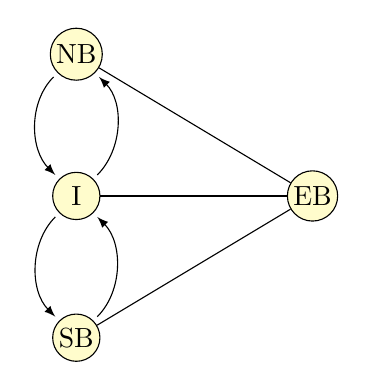
\begin{tikzpicture}[
  every node/.style={circle, draw, fill=yellow!20, minimum size=6mm, inner sep=1pt},
  >=latex
]
  % Nodes
  \node (SB) at (0,0) {SB};
  \node (I)  at (0,1.8) {I};
  \node (NB) at (0,3.6) {NB};
  \node (EB) at (3,1.8) {EB};

  % Straight edges
  \draw (SB) -- (EB);
  \draw (I)  -- (EB);
  \draw (NB) -- (EB);

  % Curved arcs with spacing from node boundaries
    \draw[->, shorten >=2pt, shorten <=2pt] (I) to[out=45, in=-45] (NB);
  \draw[->, shorten >=2pt, shorten <=2pt] (NB) to[out=225, in=135] (I);
  \draw[->, shorten >=2pt, shorten <=2pt] (SB) to[out=45, in=-45] (I);
  \draw[->, shorten >=2pt, shorten <=2pt] (I) to[out=225, in=135] (SB);

\end{tikzpicture}
\end{document}
